\chapter{Cores: the minimal structural information}\label{ch:minimal}

\Cref{thm:nerve} says that the dead-set pattern $D_A$ determines $\beta_2$. How much of $D_A$ must an observer see? This chapter measures, on the six-label census, how much \emph{count-level} information about the nerve (numbers of vertices, edges, triangles, Euler characteristics, numbers of hollow triangles) leaves uncertain about whether $\beta_2>0$, and contrasts it with a \emph{structural} reduction that preserves the answer exactly: strong collapse of the nerve to its core, followed by one $H_1$ computation. Counts are insufficient; the core is sufficient by a theorem; the core is not claimed to be minimal.

\section{Strong collapses and cores}
Let $\mathcal K$ be a finite simplicial complex. A vertex $v$ is \emph{dominated} by a vertex $w\neq v$ if every maximal simplex of $\mathcal K$ containing $v$ also contains $w$. Deleting a dominated vertex, together with all simplices containing it, is a \emph{strong collapse}; the result is a deformation retract of $\mathcal K$.
\begin{theorem}[strong collapses preserve homotopy type; \cite{BarmakMinian}]\label[theorem]{thm:barmak}
If $v$ is dominated in $\mathcal K$ then $\mathcal K\setminus v\simeq\mathcal K$ (indeed $\mathcal K$ strong-collapses onto $\mathcal K\setminus v$). Iterating until no vertex is dominated yields a complex $\mathcal K_0$, the \emph{core} of $\mathcal K$, with $\mathcal K_0\simeq\mathcal K$; the isomorphism class of the core does not depend on the order of collapses.

\end{theorem}
\begin{corollary}[the core suffices; analytic]\label[corollary]{cor:core-suffices}
For prefix-defined $A$ with $\emptyset\ne A\subsetneq S_6$, let $\mathcal C_A$ be the core of $N[D_A]$. Then $\beta_2(K_A)=\dim H_1(\mathcal C_A;\F)$ and $\beta_1(K_A)=\dim\Hh_2(\mathcal C_A;\F)$.

\end{corollary}
\begin{proof}
$N[D_A]\simeq Y_A$ by \cref{thm:nerve}, and the core is homotopy equivalent to the nerve by \cref{thm:barmak}. Homology is a homotopy invariant; the Betti formulas are \cref{thm:AD}.
\end{proof}

\section{What counts cannot see}\label{sec:D21}
Let $\mathcal P_{21}$ be the set of distinct rank-indexed dead-set patterns arising in the six-label census. The census has $346{,}859$ regimes, of which $8{,}008$ are fully admissible (there $Y_A=\emptyset$) and are excluded, leaving $338{,}851$ regimes with $219{,}145$ distinct patterns, $151$ of them with $\beta_2>0$ (carried by $158$ positive regimes). For each pattern the numbers of vertices, edges and triangles of the nerve, the Euler characteristic of its $2$-skeleton, the number of hollow triangles and the size of the strong-collapse core were computed.
\begin{table}[ht]\centering\small
\begin{tabular}{@{}lrrr@{}}\toprule
observation $O$ of the nerve & $H(Y|O)$ natural & $H(Y|O)$ balanced & classes\\ \midrule
$V=|D|$ & $0.0049$ & $0.5122$ & $57$\\
$(V,E)$ & $0.0037$ & $0.2418$ & $388$\\
Euler characteristic of the $2$-skeleton & $0.0020$ & $0.1073$ & $10{,}930$\\
number of hollow triangles & $0.0038$ & $0.1919$ & $2{,}639$\\
$(V,E,\#\text{triangles})$ & $0.0006$ & $0.0052$ & $20{,}595$\\
collapse-core size & $0.0009$ & $0.0319$ & $57$\\
(core size, hollow count) & $0.00002$ & $0.00007$ & $11{,}468$\\
collapse core, then $H_1$ & $0$ & $0$ & ---\\ \bottomrule
\end{tabular}
\caption{Exact residual uncertainty (bits) about $\beta_2>0$ over the six-label census for count-level observations of the dead-set nerve. The last row is a control: by \cref{cor:core-suffices} it computes $Y$ exactly. These values were obtained in the earlier companion computation and are not recomputed here (\cref{app:status}).}\label{tab:D21}
\end{table}
\begin{observation}[no tested count-level statistic of the nerve is sufficient; finite-exact]\label[observation]{obs:collapse}
In \cref{tab:D21} every count-level row has positive residual entropy: counts of vertices, edges, triangles, hollow triangles, the Euler characteristic and even the core size, alone or in the pairs tested, leave positives and negatives in common classes. Only the structural reduction (collapse to the core followed by $H_1$) has zero residual, and by \cref{cor:core-suffices} it does so as a theorem and not as a measurement. We do not claim that the core is the smallest possible observation, nor any out-of-sample statement beyond the census; these entropies describe a finite ensemble.
Structural facts about the cores, in the census:
\begin{itemize}[nosep]
\item Positive patterns have small cores: of the $151$, the strong-collapse core sizes are $3$ (for $105$ patterns: the bare hollow triangle), $5$ ($23$), $6$ ($6$), $7$ ($1$), $8$ ($2$), $14$ ($5$), $19$ ($1$), $20$ ($3$), $21$ ($3$) and $33$ ($2$) vertices. This distribution was recomputed exactly from the dead-set patterns of the $158$ census positives, giving the same $151$ patterns and sizes.
\item $148{,}096$ of the negative patterns collapse to a single point; the cores of the remaining negatives reach $57$ vertices but have vanishing first homology (not recomputed).
\end{itemize}

\end{observation}
\begin{figure}[ht]\centering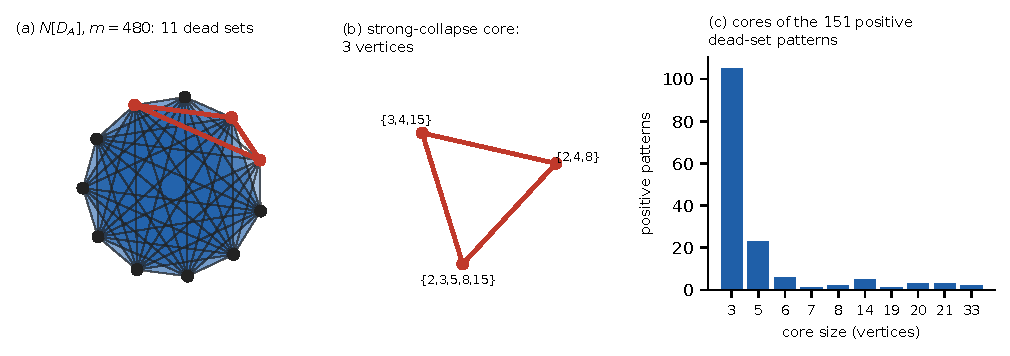
\includegraphics[width=\textwidth]{figures/fig_core.pdf}
\caption{(a)~The dead-set nerve of content $(2,3,4,5,8,15)$ at source $480$ ($11$ dead sets). (b)~Its strong-collapse core: three vertices forming the boundary of a triangle, so $\beta_2=1$. Both are drawn from the exact computation. (c)~Core sizes of the $151$ positive dead-set patterns of the census (recomputed exactly).}\label{fig:collapse}
\end{figure}
The question ``what is the minimal structural information that determines whether a hole exists?'' has three different answers depending on the observer. \emph{Without structure} (counts only), no tested statistic suffices (\cref{tab:D21}). \emph{With the dead-set pattern}, the answer is determined (\cref{thm:nerve}). \emph{With a homotopy-preserving reduction}, a hollow triangle in $105$ of the $151$ positive patterns is the entire information. No universal optimality is claimed: a smaller sufficient observation of the pattern could exist, and no lower bound is proved.
\begin{proposition}[counts cannot see the cycle --- a certified instance; finite-exact]\label[proposition]{prop:counts-fail}
The two systems of \cref{prop:pair} at sources $2520$ and $3780$ have the same number ($5$) of dead sets and the same $N$, $E$, $Q$, $h_1$; their nerves have the same number of vertices ($5$), but differ in $\beta_2$ ($1$ vs $0$). The nerves have different edge sets, and the first one contains a non-bounding hollow triangle.

\end{proposition}
A hollow triangle is a triple of forbidden prefix sets, pairwise compatible, with no prefix set related to all three. By \cref{obs:cycle-census} it occurs in $288$ of the $290$ positives and also in many negatives, where it always bounds. The difference between a bounding and a non-bounding hollow triangle is homological rather than local.
